%-------------------------------------------------------------------------------
%	DIRC TECHNOLOGY CHAPTER
%-------------------------------------------------------------------------------
\label{ch:components}
The validation of key components of the DIRC for an EIC in vital to show that the Geant4 simulation package produces results expected for the real detector. However, due to budget restraints it was not possible to build or otherwise procure a full scale prototype of the envisioned EIC DIRC discussed in Chapter \ref{ch:eicdirc} (e.g. $2\unit{mm}$ pixel MCP-PMTs are not available on the market). Instead a series of test bench measurements were made for both the NLaK33 material of the 3-layer lens and for the performance of similar MCP-PMTs in high magnetic field environments.
The FDIRC R\&D program found that implementing focusing into the design of a DIRC improves performance and allows for a smaller, more compact expansion volume. A DIRC at EIC hopes to take advantage of this by utilizing a new 3-layer spherical lens design, a schematic of which is shown in Figure \ref{fig:3CS_schematic}a. 

\begin{figure}[ht]
	\centering
	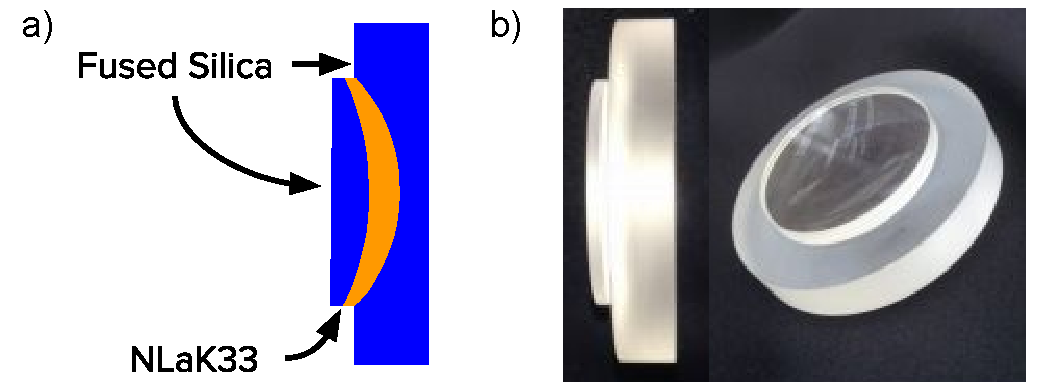
\includegraphics[width=\textwidth]{3CS_schematic.pdf}
	\caption{Schematic drawing of the 3-layer lens design with two layers of fused silica sandwiching a layer of high refractive index NLaK33 glass (a), and a side and front view of a prototype lens built for testing (b).}
	\label{fig:3CS_schematic}
\end{figure}



%-------------------------------------------------------------------------------
%	3-LAYER LENS OPTICS SECTION
%-------------------------------------------------------------------------------
\section{Optical Properties of 3-Layer Lens}


%-------------------------------------------------------------------------------
%	NLAK33 RAD HARDNESS SECTION
%-------------------------------------------------------------------------------
\section{Radiation Hardness of NLaK33 Material}

%-------------------------------------------------------------------------------
%	HIGH-B TESTS SECTION
%-------------------------------------------------------------------------------
\section{Performance of MCP-PMTs in High Magnetic Field}